\documentclass[tikz,border=9pt]{standalone}
\usepackage{tikz}
\begin{document}
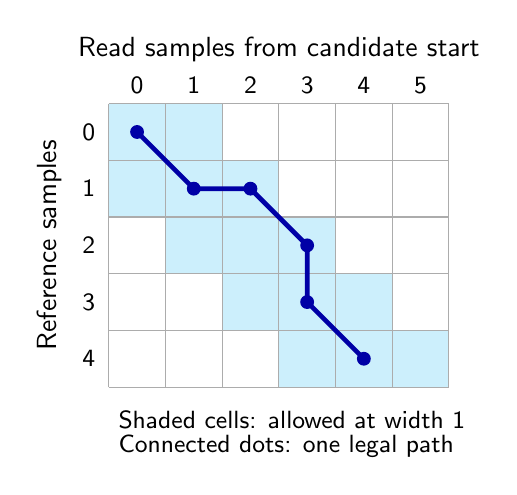
\begin{tikzpicture}[x=.72cm,y=.72cm,font=\sffamily]
  \foreach \i in {0,...,4}{
    \foreach \j in {0,...,5}{
      \ifnum\numexpr\i-\j\relax<2
        \ifnum\numexpr\j-\i\relax<2
          \fill[cyan!20] (\j,-\i) rectangle ++(1,-1);
        \fi
      \fi}}
  \draw[step=1,gray!65] (0,0) grid (6,-5);
  \foreach \j in {0,...,5} \node at (\j+.5,.32) {\small\j};
  \foreach \i in {0,...,4} \node at (-.35,-\i-.5) {\small\i};
  \node at (3,.96) {Read samples from candidate start};
  \node[rotate=90] at (-1.05,-2.5) {Reference samples};
  \draw[blue!65!black,line width=1.7pt] (.5,-.5)--(1.5,-1.5)--(2.5,-1.5)
      --(3.5,-2.5)--(3.5,-3.5)--(4.5,-4.5);
  \foreach \p in {(.5,-.5),(1.5,-1.5),(2.5,-1.5),(3.5,-2.5),(3.5,-3.5),(4.5,-4.5)}
      \fill[blue!65!black] \p circle (2.5pt);
  \node[anchor=west,font=\sffamily\small] at (0,-5.58) {Shaded cells: allowed at width 1};
  \node[anchor=west,font=\sffamily\small] at (0,-6.04) {Connected dots: one legal path};
\end{tikzpicture}
\end{document}
